% !TeX spellcheck = it_IT
\newpage
\section{Verifica e validazione}
Verifica e validazione sono attività di \textbf{software quality assurance} e sono parte integrante del processo software da svolgere in ogni fase per confermare che \textbf{processo} e \textbf{prodotto} rispettino i requisiti di qualità.
\begin{center}
	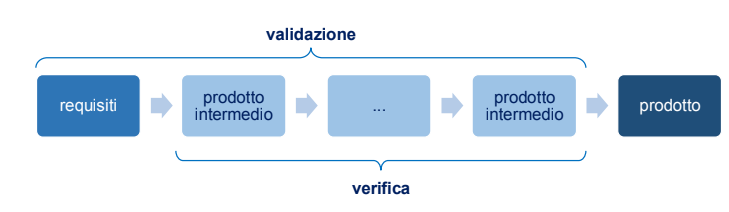
\includegraphics[scale=.4]{vv}
\end{center}
La \textbf{convalida} o validazione risponde alla domanda "Stiamo costruendo il sistema che serve all'utente?" mentre la \textbf{verifica} risponde a "Stiamo costruendo un sistema che rispetta le specifiche?".
\begin{center}
	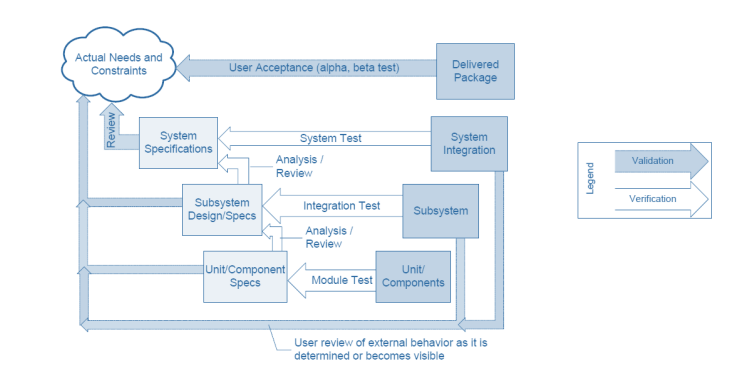
\includegraphics[scale=.5]{vorv}
\end{center}

\subsection{Limiti}
Un risultato fondamentale per la verifica e la validazione è quello dei problemi \textbf{non decidibili}: algoritmi per i quali non esiste alcun algoritmo in grado di dare una risposta in tempo finito su tutte le istanze del problema.

\begin{definition}[Halting problem]
	Non esiste un programma $P$ che per ogni programma $Q$ e input $D$ dice se il programma $Q$ sull'input $D$ termina o meno.
\end{definition}

Un altro esempio di indecidibilità è dire se due programmi, dati gli stessi input, producono lo stesso risultato.

\paragraph{Triple di Hoare}
Una tecnica per la verifica e validazione è tramite le triple di Hoare, basata sulla logica del prim'ordine. Quest'ultima però è \textbf{indecidibile} dato che, data una formula $F$ non esiste un algoritmo per decidere in tempo finito se questa è verificata. È possibile enumerare le formule valide ma non è detto che si dimostri $F$ o $\neg F$.

\subsubsection{Difficoltà}
Le difficoltà principali per la verifica e la validazione sono:
\begin{itemize}
	\item I \textbf{requisiti} di qualità sono \textbf{diversi} tra loro
	\item Un prodotto software è in \textbf{costante evoluzione}
	\item I guasti hanno una distribuzione irregolare
	\item Verifica e validazione sono \textbf{non-lineari}: se una procedura ordina correttamente $X$ elementi non è detto che ne ordini correttamente anche $Y \neq S$
	\item Approcci diversi possono introdurre errori diversi, e.g. il SW distribuito può portare a \textit{deadlock} o \textit{race conditions} mentre quello object-oriented problemi dovuti al \textit{polimorfismo} o al \textit{binding dinamico}
\end{itemize}

\subsection{Progettazione}
I progettisti di questa fase devono:
\begin{itemize}
	\item Scegliere e programmare la giusta combinazione di tecniche per raggiungere il \textbf{livello richiesto di qualità} entro i \textbf{limiti di costo}
	\item Progettare una soluzione specifica che si adatti al \textbf{problema}, ai \textbf{requisiti} e all'\textbf{ambiente di sviluppo}
\end{itemize}

\subsubsection{Quando iniziare e finire}
Verifica e validazione non sono solo una fase finale. Iniziano dallo \textbf{studio di fattibilità}, dove bisogna tenere conto di \textbf{qualità richieste} e \textbf{impatto sul costo} complessivo. Inoltre permettono di svolgere attività correlate alla qualità come:
\begin{itemize}
	\item Analisi del rischio
	\item Definizione delle misure per valutare e controllare la qualità durante le diverse fasi di sviluppo
	\item Valutazione dell'impatto di nuove funzionalità e nuovi requisiti di qualità
	\item Valutazione economica delle attività di controllo della qualità, quali costi e tempi di sviluppo
\end{itemize}
Inoltre continuano anche \textbf{dopo il rilascio} ed includono attività di \textbf{manutenzione}, tra cui:
\begin{itemize}
	\item Analisi delle modifiche ed estensioni
	\item Generazione di nuove suite di test per le funzionalità aggiuntive
	\item Ripetizione dei test per verificare la non regressione delle funzionalità precedenti a seguito di modifiche ed estensioni
	\item Rilevamento ed analisi dei guasti
\end{itemize}

\subsubsection{Quali tecniche}
Non basta una sola tecnica ma è meglio combinarne diverse di analisi e testing, basandosi su diversi aspetti e sulle diverse fasi in cui ci si trova:
\begin{itemize}
	\item \textbf{Efficacia diversa}: per diverse classi di difetto (e.g. analisi statica per identificazione di race conditions)
	\item \textbf{Applicabilità} in \textbf{diverse fasi} del processo di sviluppo (e.g. ispezione per la convalida dei requisiti iniziali e testing per la validazione del prodotto finale)
	\item \textbf{Differenze negli scopi} (e.g. test statistico per misurare l'affidabilità)
	\item \textbf{Compromessi} in termine di costi ed affidabilità (e.g. tecniche costose solo per i requisiti di sicurezza)
\end{itemize}

\subsubsection{Valutazione del prodotto pronto}
Per valutare un prodotto pronto bisogna individuare e definire bene le misure di qualità del software di interesse:
\begin{itemize}
	\item \textbf{Disponibilità} in termini di tempo di esecuzione in rapporto con il tempo in cui il sistema non è disponibile
	\item \textbf{Tempo medio tra i guasti}
	\item \textbf{Affidabilità} misurata come la percentuale di operazioni che terminano con successo
\end{itemize}
Esistono due tipologie di test:
\begin{itemize}
	\item \textbf{Alfa test}: eseguiti da sviluppatori o utenti selezionati, in ambiente controllato ed osservati dall'organizzazione dello sviluppo
	\item \textbf{Beta test}: eseguiti da utenti reali nel loro ambiente e senza interferenze o monitoraggio ravvicinato
\end{itemize}


\subsubsection{Controllare release successive}
Dopo la consegna del prodotto finito ci sono comunque attività che devono essere fatte:
\begin{itemize}
	\item Test ed analisi di codice nuovo o modificato
	\item Ripetizione dei \textbf{test di sistema}
	\item \textbf{Memorizzazione dei bug} trovati
	\item Testi di \textbf{regressione}
	\item Distinzione tra cambiamenti di versione \textit{major} e \textit{minor}
\end{itemize}

\subsubsection{Migliorare il processo}
Per migliorare il processo si devono identificare e rimuovere i punti deboli all'interno del processo di sviluppo e quelli del test e dell'analisi (che non permettono di individuare i primi).

\subsection{Terminologia}
\begin{definition}[Malfunzionamento]
	Il sistema SW a runtime non si comporta secondo le specifiche. Ha natura \textbf{dinamica} e può essere osservato solo mediante esecuzione. È causato da uno o più difetti.
\end{definition}
\begin{definition}[Difetto]
	Anomalia, bug o fault nel codice del sistema SW. Appartiene alla struttura statica del programma. L'atto di correzione è definito \textbf{debugging} o \textbf{bug fixing}. Può causare uno o più malfunzionamenti e se non ne causa si dice che è \textbf{latente} (e.g. in un flusso che non viene quasi mai eseguito o difetti che si annullano a vicenda).
\end{definition}

\begin{definition}[Errore]
	È la causa del difetto. Un errore umano nella comprensione o risoluzione dei problemi o nell'uso di strumenti.
\end{definition}

\subsection{Verifica statica}
La verifica statica non prevede l'esecuzione del programma e si divide in due tipi di metodi:
\begin{itemize}
	\item \textbf{Manuali}: basati sulla \textit{desk-check} (lettura del codice). Sono i più comuni e più o meno formalmente documentati.
	\item \textbf{Formali} o supportati da \textbf{strumenti}:
	\begin{itemize}
		\item Model checking
		\item Esecuzione simbolica
		\item Interpretazione astratta
		\item Theorem proving
	\end{itemize}
\end{itemize}

\subsubsection{Desk check}
Il desk-check è l'analisi manuale di programmi software volta a capire cosa facciano e/o ad identificare errori logici che potrebbero occorrere durante la loro esecuzione. Esistono due metodologie \textbf{pratiche} (lettura del codice e dipendenti dall'esperienza) e \textbf{complementari} tra loro: \textit{inspection} e \textit{walkthrough}.
\paragraph{Inspection} Si esegue una lettura mirata del codice guidata da una checklist. L'biettivo è di rivelare la presenza di difetti focalizzando la ricerca su aspetti ben definiti (error guessing) (e.g. off-by-one error). La ricerca viene portata avanti dagli \textbf{ispettori}. Si divide in quattro fasi:
\begin{enumerate}
	\item \textbf{Pianificazione}
	\item Definizione della \textbf{checklist}. Sono frutto dell'esperienza degli ispettori. Tipicamente contengono aspetti che non sono controllabili in maniera automatica e sono aggiornate ad ogni iterazione.
	\item \textbf{Lettura} del codice
	\item \textbf{Correzione} dei difetti
\end{enumerate}

\paragraph{Walkthrough} Si esegue una lettura critica del codice con l'obiettivo di rivelare la presenza di difetti percorrendo il codice e simulandone l'esecuzione. È eseguita da gruppi misti di \textit{ispettori} e programmatori. È più completo dell'inspection ma meno rapido. Si divide in tre fasi:
\begin{enumerate}
	\item \textbf{Pianificazione}
	\item \textbf{Lettura} del codice
	\item \textbf{Correzione} dei difetti
\end{enumerate}

Il desk-check è \textbf{pratico} ed \textbf{intuitivo}, rendendolo ideale per alcune caratteristiche di qualità. Inoltre \textbf{conviene economicamente}: i costi dipendono dalla dimensione del codice e sono quindi bassi per quanto riguarda l'infrastruttura. Permette una buona prevedibilità dei risultati.

\subsubsection{Metodi formali}
I metodi formali sono tecniche basate sulla dimostrazione formale di correttezza di un modello finito (che ha dimostrazione possibile) e istanziazione del modello.
\begin{example}[Two-phase locking]
	Il protocollo two-phase locking, una volta dimostrato corretto e istanziato correttamente, garantisce assenza di malfunzionamenti dovuti alla race condition. Allo stesso tempo però ci sono applicazioni che non lo usano ma che sono comunque corrette e bisogna anche dimostrare che il programma applichi il protocollo correttamente (comunque più facile che provare l'assenza di malfunzionamenti in generale).
\end{example}
Esempi di metodi formali sono le \textbf{triple di Hoare}, il \textbf{B method} e il \textbf{model checking.}
\begin{figure}[!h]
	\hfill
	\subfigure[Triple di Hoare]{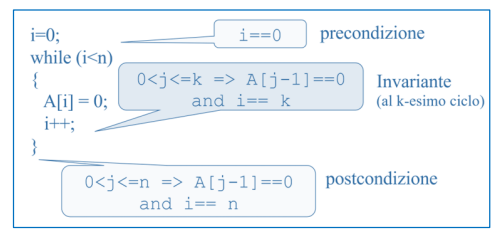
\includegraphics[width=7cm]{hoare}}
	\hfill
	\subfigure[Model checking]{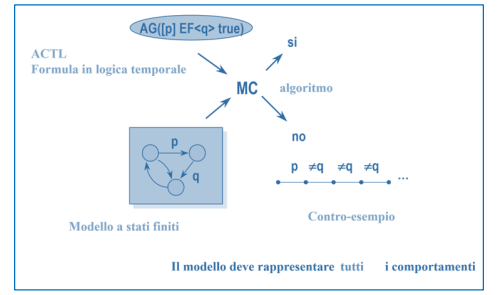
\includegraphics[width=7cm]{modelcheck}}
\end{figure}

\subsection{Verifica dinamica}
La verifica dinamica, o \textbf{testing}, si compone di quattro fasi:
\begin{enumerate}
	\item \textbf{Progettazione}: input, output atteso e ambiente di esecuzione del test
	\item \textbf{Esecuzione} del codice
	\item \textbf{Analisi} dei risultati, ovvero il confronto tra l'output ottenuto e quello atteso
	\item \textbf{Debugging}
\end{enumerate}
Livelli diversi della fase di progettazione richiedono testing diversi.
\begin{center}
	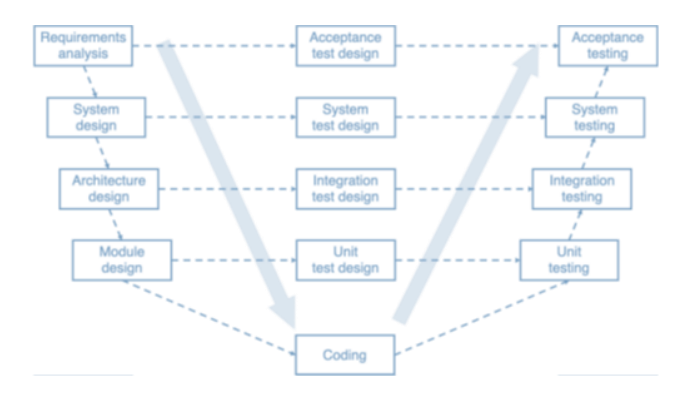
\includegraphics[scale=.5]{testlvl}
\end{center}

\subsubsection{Progettazione}
È fondamentale poter ripetere una sessione di test in condizioni immutate, ovvero:
\begin{itemize}
	\item In un \textbf{ambiente definito}, sia per l'HW che per le condizioni
	\item Con \textbf{casi di prova} definiti, ovvero con input predefiniti e comportamenti (o output) attesi
	\item Con \textbf{procedure definite}
\end{itemize}

\begin{definition}[Caso di prova]
	Un caso di prova è una tripla
	\begin{equation*}
		\langle \text{input}, \text{output\_atteso}, \text{ambiente}\rangle
	\end{equation*}
\end{definition}
\noindent Per la progettazione servono:
\begin{itemize}
	\item \textbf{Test obbligation}: specifica di casi di test utili a verificare proprietà ritenute importanti. Si possono definire in diversi modi:
	\begin{itemize}
		\item \textbf{Black box}: a partire dalle \textit{funzionalità} indicate nella specifica del software, per evidenziarne malfunzionamenti.
		\item \textbf{White box}: a partire dalla struttura, guardando il codice, per esercitarlo indipendentemente dalle funzionalità
		\item A partire dal \textit{modello} del programma utilizzato nella specifica o progettazione oppure derivato dal codice
		\item A partire da \textit{fault ipotetici}, cercando difetti ipotizzati o bug comuni
	\end{itemize}
	\item \textbf{Criteri} per definire l'\textbf{adeguatezza} di un insieme di casi di test. Sostanzialmente è un insieme di \textit{test obbligation}. Si considera \textbf{soddisfatto} se tutti i test hanno successo e se ogni test obbligation è soddisfatta da almeno un caso di test nell'insieme scelto.
\end{itemize}

\begin{definition}[Batterie di prove]
	Una batteria di prova, o test suite, è un insieme o sequenza di casi di prova.
\end{definition}
\begin{definition}[Procedura di prova]
	Procedure automatiche e non per eseguire, registrare, analizzare e valutare i risultati di una batterie di prove. Si articola in più fasi:
	\begin{enumerate}
		\item Definizione dell'obiettivo della prova
		\item Progettazione della prova: scelta e definizione dei casi
		\item Realizzazione dell'ambiente di prova: driver e stub da realizzare, ambienti da controllare, strumenti per la registrazione dei dati da analizzare
		\item Esecuzione della prova
		\item Analisi dei risultati alla ricerca di evidenza di malfunzionamenti
		\item Valutazione della prova
	\end{enumerate}
\end{definition}
\noindent Inoltre, per eseguire un test, è necessario del codice aggiuntivo chiamato \textbf{scaffolding}, che può includere:
\begin{itemize}
	\item \textbf{Driver} di test che sostituiscono il chiamante
	\item \textbf{Stub} o \textbf{mock} che sostituiscono a funzionalità del chiamante
	\item \textbf{Test harness}, che sostituiscono parti dell'ambiente di distribuzione
	\item \textbf{Tool} per gestire l'esecuzione e la registrazione di risultati
\end{itemize}
\begin{example}
	Se il metodo $A$ usa $B$ che usa $C$ e voglio testare $B$, devo costruire del codice che simula $A$ (driver) e che simula $C$ (stub).
\end{example}

\subsubsection{Black box}
La strategia per la generazione dei casi con metodi black box consiste in:
\begin{enumerate}
	\item Separare le funzionalità da testare, e.g. basandosi sui casi d'uso
	\item Derivare un insieme di casi di test per ogni funzionalità:
	\begin{itemize}
		\item Per ogni tipo di parametro di input si individuano dei valori da testare sfruttando varie tecniche
		\begin{itemize}
			\item \textbf{Metodo statistico}: i casi di test vengono selezionati in base alla distribuzione di probabilità degli input del programma (il test viene fatto sugli input più probabili). È automatizzabile ma è difficile e costoso calcolare il risultato atteso (\textbf{problema dell'oracolo})
			\item \textbf{Partizione in categorie}: il dominio degli input è ripartito in categorie o classi di equivalenza. Due input appartengono alla stessa se, in base ai requisiti, dovrebbero produrre lo stesso comportamento del programma. È conveniente solo se il numero dei possibili comportamenti è molto inferiore alle possibili configurazioni in ingresso. Si basa su un'affermazione generalmente plausibile ma non vera in assoluto.
			\item \textbf{Frontiera}: si individuano i valori limite rispetto alle classi di equivalenza e rispetto al tipo degli input. Spesso è proprio intorno a questi valori che si nascondono difetti del codice. Molto efficace quando la frontiera è un punto di discontinuità.
			\item \textbf{Casi non validi}: per ogni input si definiscono i casi che devono generare un errore
			\item \textbf{Random}: si genera un insieme grande a piacere di valori in modo automatico e casuale. È a costo zero man on sempre è ripetibile. È applicabile se l'esecuzione costa poco.
			\item \textbf{Catalogo}: l'esperienza acquisita nel definire i casi di test può essere collezionata in un catalogo per rendere più veloce il processo e ridurre l'errore umano. Si elencano tutti i casi che devono essere considerati per ciascun tipo di variabile.
		\end{itemize}
		\item Per l'insieme di parametri si usano tecniche di \textbf{test combinatorio}. Dato che al crescere del numero degli input il prodotto cartesiano dei casi di test individuati può diventare ingestibile a causa dell'esplosione combinatoria, vediamo alcune tecniche per gestire la generazione dei casi di test:
		\begin{itemize}
			\item \textbf{Vincoli}: si introducono per limitare il numero di test ottenuti. Possono essere:
			\begin{itemize}
				\item Di \textit{errore}: un solo caso di errore (input non valido) per ogni posizione
				\item Di \textit{proprietà}: si definiscono proprietà comuni per classi di equivalenza diverse che poi vengono usate per guidare la combinazione dei test
				\item \textit{Singoletti}: si testa un solo valore per uno o più parametri
			\end{itemize}
			\item \textbf{Pairwise testing}: si basa su coppie di variabili generando tutte le combinazioni solo per i sottoinsiemi di due, e in generale per $k$ variabili con $k<n$
			
			\begin{note}
				La generazione efficiente di combinazioni che coprano tutte le coppie è impossibile da fare a mano per molti parametri con molti valori ma può essere fatta con euristiche.
			\end{note}
		\end{itemize}
	\end{itemize}
\end{enumerate}

\subsubsection{White box}
I criteri white-box, anche detti \textbf{strutturali}, si basano sulla struttura del codice ed aiutano ad aggiungere altri test oltre a quelli generati con criteri \textit{funzionali}.\\
Questi criteri sono definiti per classi particolari di elementi, quali \textit{comandi}, \textit{branch} e \textit{condizioni}, e richiedono che i test esercitino \textbf{tutti} quegli elementi del programma.

\begin{definition}[Grafo di flusso]
	Il grafo di flusso (flow-chart) definisce a partire dal codice la struttura dello stesso. Identifica le sue parti e come sono collegate tra loro.
\end{definition}

\paragraph{Criteri di copertura} Nel contesto dei grafi di flusso abbiamo alcuni tipi di coperture che dobbiamo rispettare:
\begin{itemize}
	\item \textbf{Comandi}: si identificano valori di input che esercitino tutti i comandi, cercando di minimizzare il numero di test a parità di copertura. L'adeguatezza della copertura si misura con:
	\begin{equation*}
		\frac{\text{numero di comandi esercitati}}{\text{numero totale di comandi}}
	\end{equation*}
	\begin{note}
		La coverage non è monotona rispetto alla dimensione dell'insieme di test.
	\end{note}
	\item \textbf{Decisioni}: si identificano valori di input che esercitino tutti i rami di ogni condizione. L'adeguatezza si misura con:
	\begin{equation*}
		\frac{\text{numero di rami esercitati}}{\text{numero totale di rami}}
	\end{equation*}
	In particolare è utile garantire la copertura delle \textbf{condizioni semplici}: per ogni condizione semplice $CS$ in un programma $P$ un insieme di test $T$ contiene contiene un test per cui $CS$ vale \textit{true} e uno per cui vale \textit{false}. Si misura in:
	\begin{equation*}
		\frac{\text{numero di valori assunti dalle condizioni semplici}}{2 \cdot\text{numero di condizioni semplici}}
	\end{equation*}
	Date $n$ condizioni semplici ci sono $2^n$ condizioni possibili da testare.
	\item \textbf{Cammini}: si identificano tutti i valori di input per esercitare tutti i cammini possibili. In presenza di cicli il numero è potenzialmente infinito e quindi si implementano casi di test che esercitino il ciclo:
	\begin{itemize}
		\item Zero volte
		\item Esattamente una volta
		\item Più di una volta
	\end{itemize}
\end{itemize}

\subsubsection{Fault-based}
Il fault-based testing si basa sull'ipotizzare dei difetti potenziali nel codice in questione e nella creazione/valutazione di una test-suite che li rilevi.\\

La tecnica più nota è quella \textbf{mutazionale}: dato un programma $P$ esercitato su una batteria di test $T$ e corretto rispetto ad essa, introduciamo dei difetti (\textbf{mutazioni}) in $P$ ottenendo $P'$. Si ripetono poi i test sul nuovo programma e si verifica:
\begin{itemize}
	\item se i difetti introdotti non sono rilevati (\textbf{sopravvivono}), $T$ non era sufficientemente buona oppure era equivalente al programma originale
	\item se sono rilevati (vengono \textbf{uccisi}), abbiamo maggior fiducia in $T$
\end{itemize}
Alcuni esempi di mutazioni:
\begin{itemize}
	\item \textit{crp}: sostituzione di costante per un'altra
	\item \textit{ror}: sostituzione dell'operatore relazionale
	\item \textit{vie}: eliminazione dell'inizializzazione di una variabile
	\item \textit{lrc}: sostituzione di un operatore logico
	\item \textit{abs}: inserimento di un valore assoluto
\end{itemize}
\begin{note}
	Una mutazione è \textbf{valida} se sintatticamente corretta e \textbf{utile} se è valida e non facilmente distinguibile dal programma originale.
\end{note}
L'efficacia di un test mutazionale si misura con:
\begin{equation*}
	\frac{\text{numero di mutanti uccisi}}{\text{numero totale di mutanti}}
\end{equation*}

\begin{observation}
	I test mutazionali si applicano in congiunzione con altri criteri di test già realizzati e possono essere completamente automatizzati.
\end{observation}

\subsubsection{Oracolo}
Un oracolo è uno strumento o metodologia in grado di generare i risultati attesi di un test case. Fornisce un punto di riferimento per valutare la \textbf{correttezza del sistema} durante il testing ed è cruciale per garantire la \textbf{qualità del software} e la \textbf{corretta individuazione} di eventuali difetti.\\
Per trovare i risultati attesi ci sono diverse tecniche:
\begin{itemize}
	\item Ricavarli dalle \textbf{specifiche} formali ed eseguibili
	\item \textbf{Inversione} delle funzioni, in particolare quando:
	\begin{itemize}
		\item la funzione inversa è più facile o disponibile
		\item possiamo partire dall'output e trovare l'input
		\item limitazione per difetti di approssimazione
	\end{itemize}
	\item \textbf{Versioni precedenti} dello stesso codice
	\item \textbf{Versioni multiple} indipendenti sviluppate ad hoc o preesistenti back-to-back
	\item \textbf{Semplificazione} dei dati in \textbf{input}, ad esempio ipotizzando un comportamento costante o usando risultati noti o calcolabili con altri mezzi
	\item \textbf{Semplificazione} dei \textbf{risultati} tramite vincoli tra input e output e invarianti sulle uscite
\end{itemize}

\subsection{Test di sistema}
Vediamo le varie tipologie di test di sistema:
\begin{itemize}
	\item \textbf{Facility}: test delle funzionalità per verificare che quelle stabilite nei requisiti siano state realizzate correttamente
	\item \textbf{Security}: controlla l'efficacia dei meccanismi di sicurezza
	\item \textbf{Usability}: controlla la facilità d'uso del prodotto da parte dell'utente finale e si compone di \textit{prodotto}, \textit{documentazione}, \textit{livello di competenza} dell'utente e \textit{caratteristiche operative dell'ambiente d'uso}
	\item \textbf{Performance}: controlla l'efficienza di un sistema rispetto ai tempi di elaborazione e di risposta
	\item \textbf{Load}: controlla l'efficienza di un sistema con il carico di lavoro massimo previsto dai requisiti e consente di individuare malfunzionamenti che non si presentano in condizioni normali
	\item \textbf{Stress}: controlla la capacità di recovery del sistema dopo un fallimento causato dall'esplicito superamento dei limiti operativi previsti dai requisiti
	\item \textbf{Storage use}: test di utilizzo della memoria persistente, controlla la sua efficienza di utilizzo
	\item \textbf{Configuration}: controlla che il sistema funzioni nelle configurazioni previste
	\item \textbf{Compatibility}: controlla la compatibilità del sistema con altri software
\end{itemize}